\documentclass{article}
\usepackage[margin=1in]{geometry}
\usepackage{graphicx} % Required for inserting images
\usepackage{tabularray}
\usepackage{float}
\usepackage{codehigh}
\usepackage{lscape}
\usepackage{adjustbox}
\usepackage[normalem]{ulem}
\UseTblrLibrary{booktabs}
\UseTblrLibrary{siunitx}
\newcommand{\tinytableTabularrayUnderline}[1]{\underline{#1}}
\newcommand{\tinytableTabularrayStrikeout}[1]{\sout{#1}}
\NewTableCommand{\tinytableDefineColor}[3]{\definecolor{#1}{#2}{#3}}

\begin{document}

\begin{figure}
\centering
\caption{Graph 1}
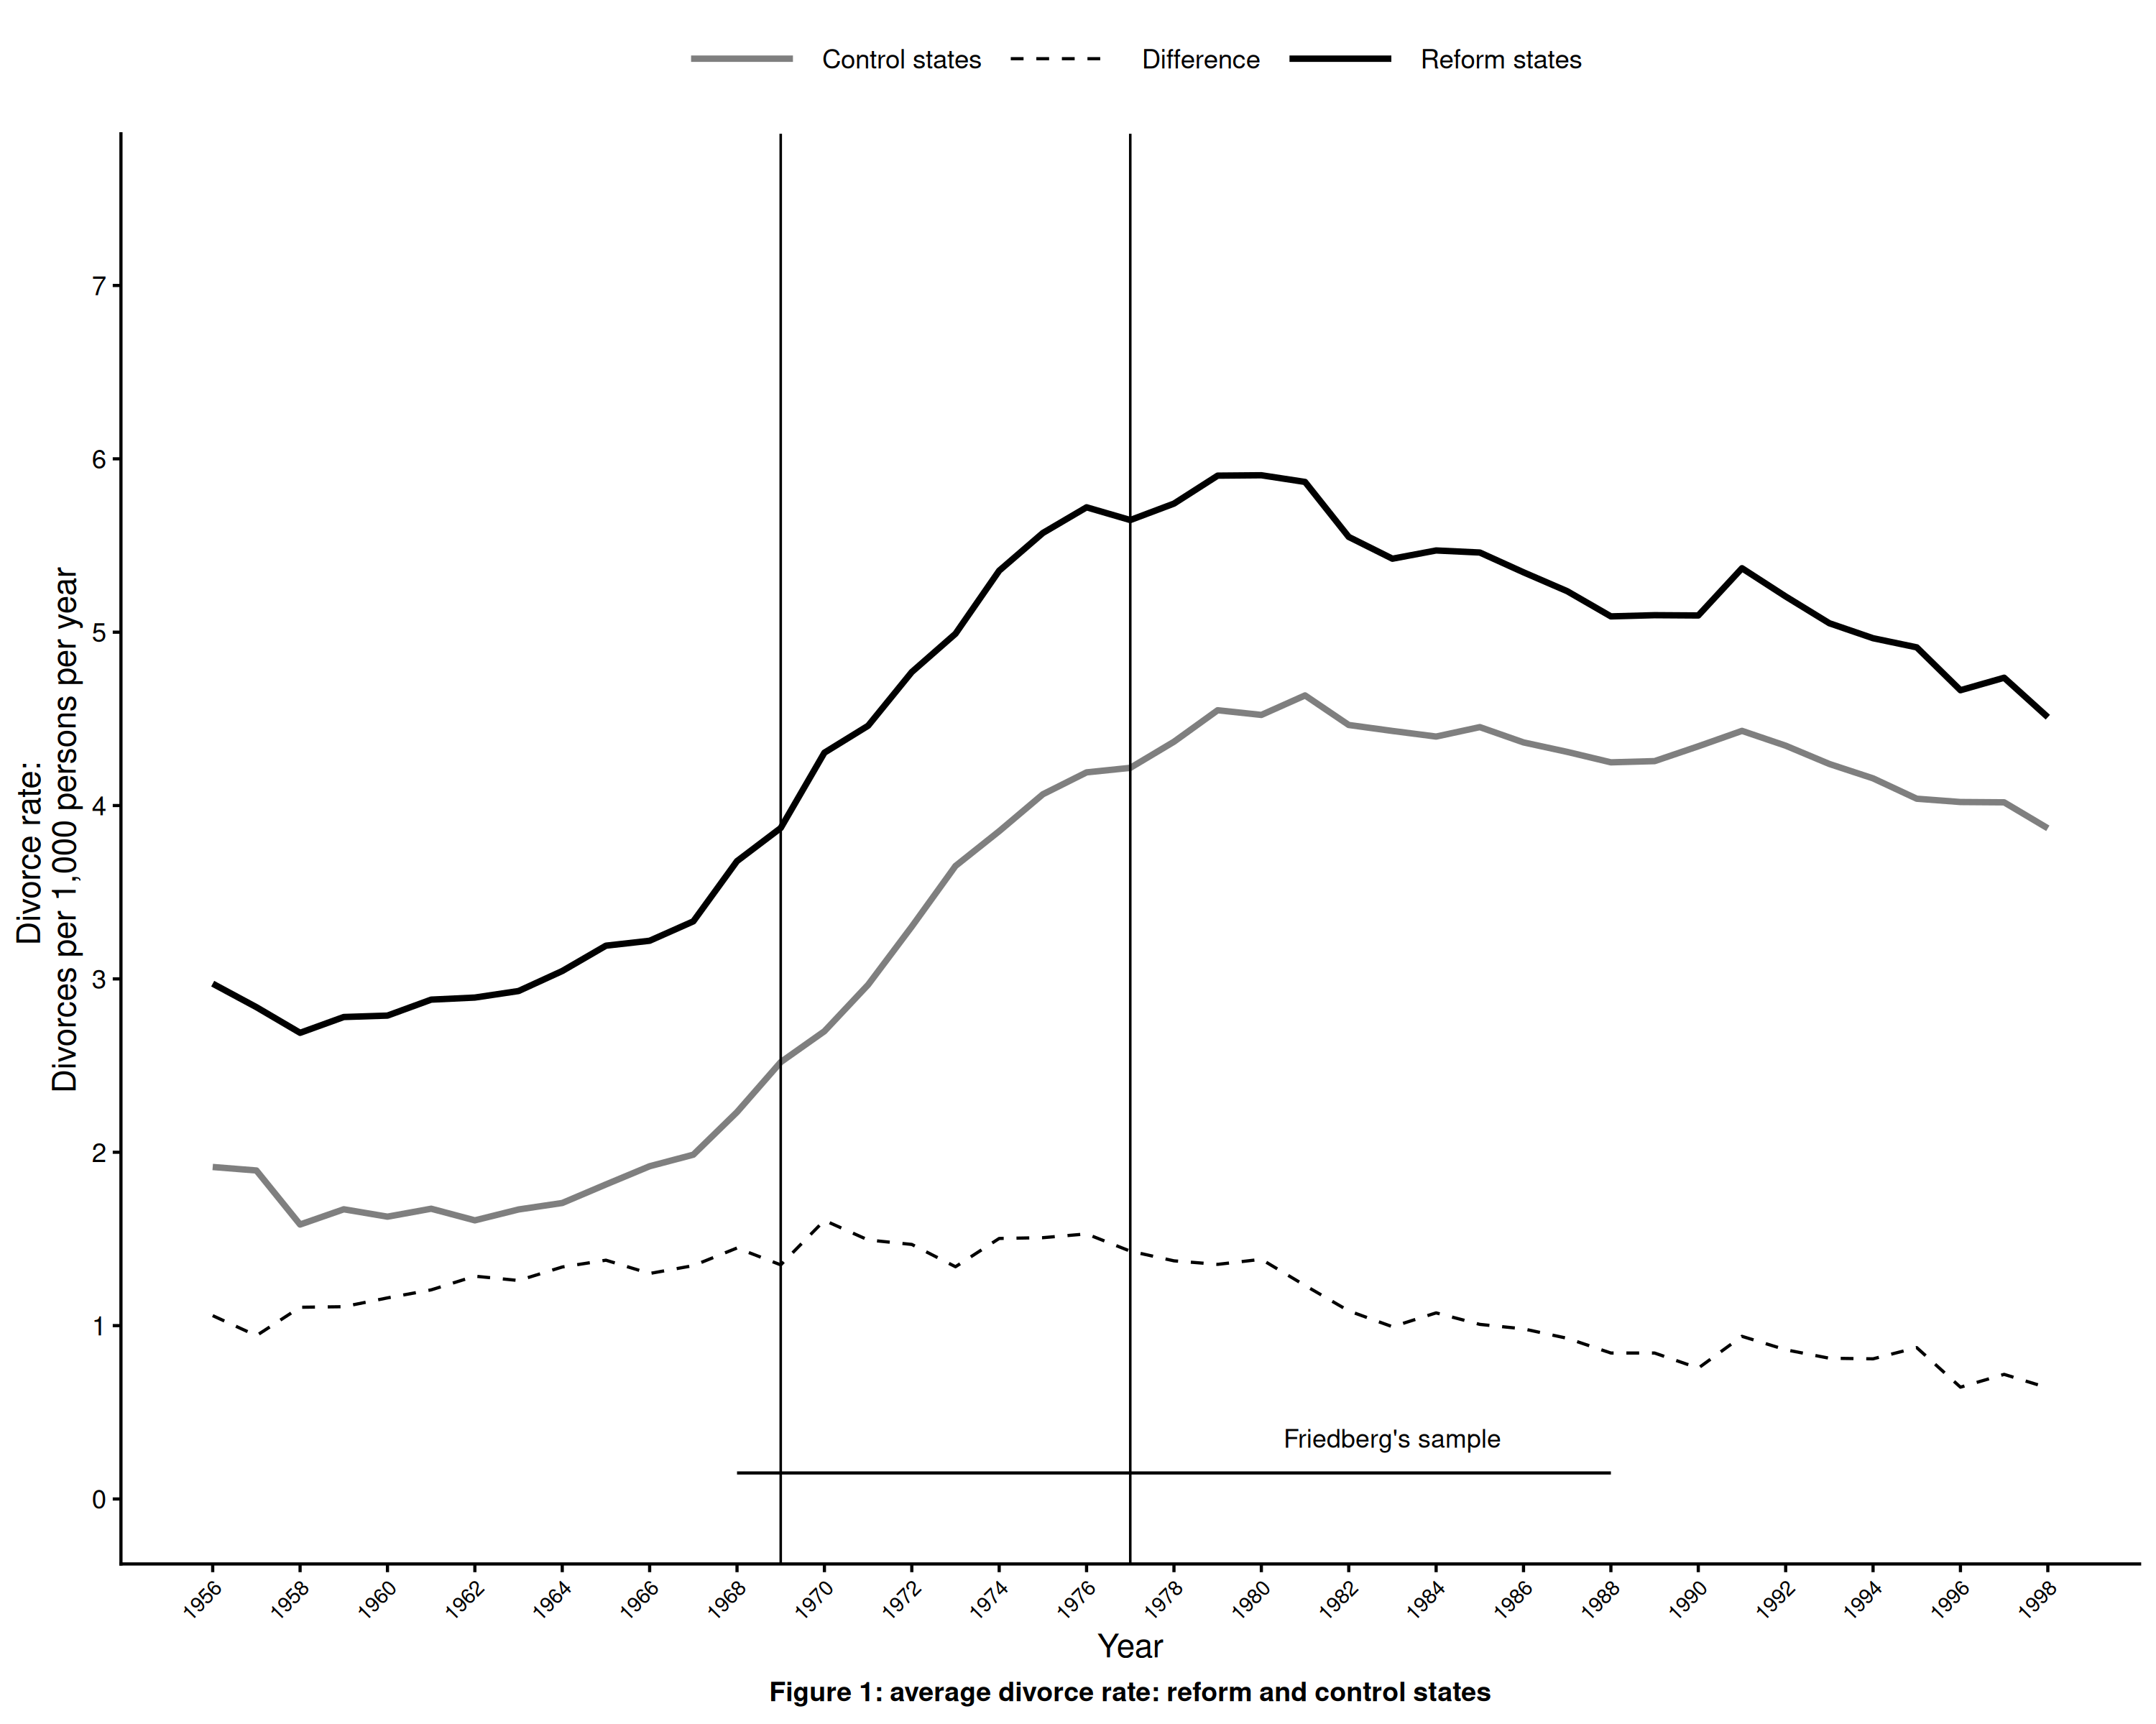
\includegraphics[scale=0.5]{graph1.png}
\end{figure}

\begin{figure}
\centering
\caption{Graph 2}
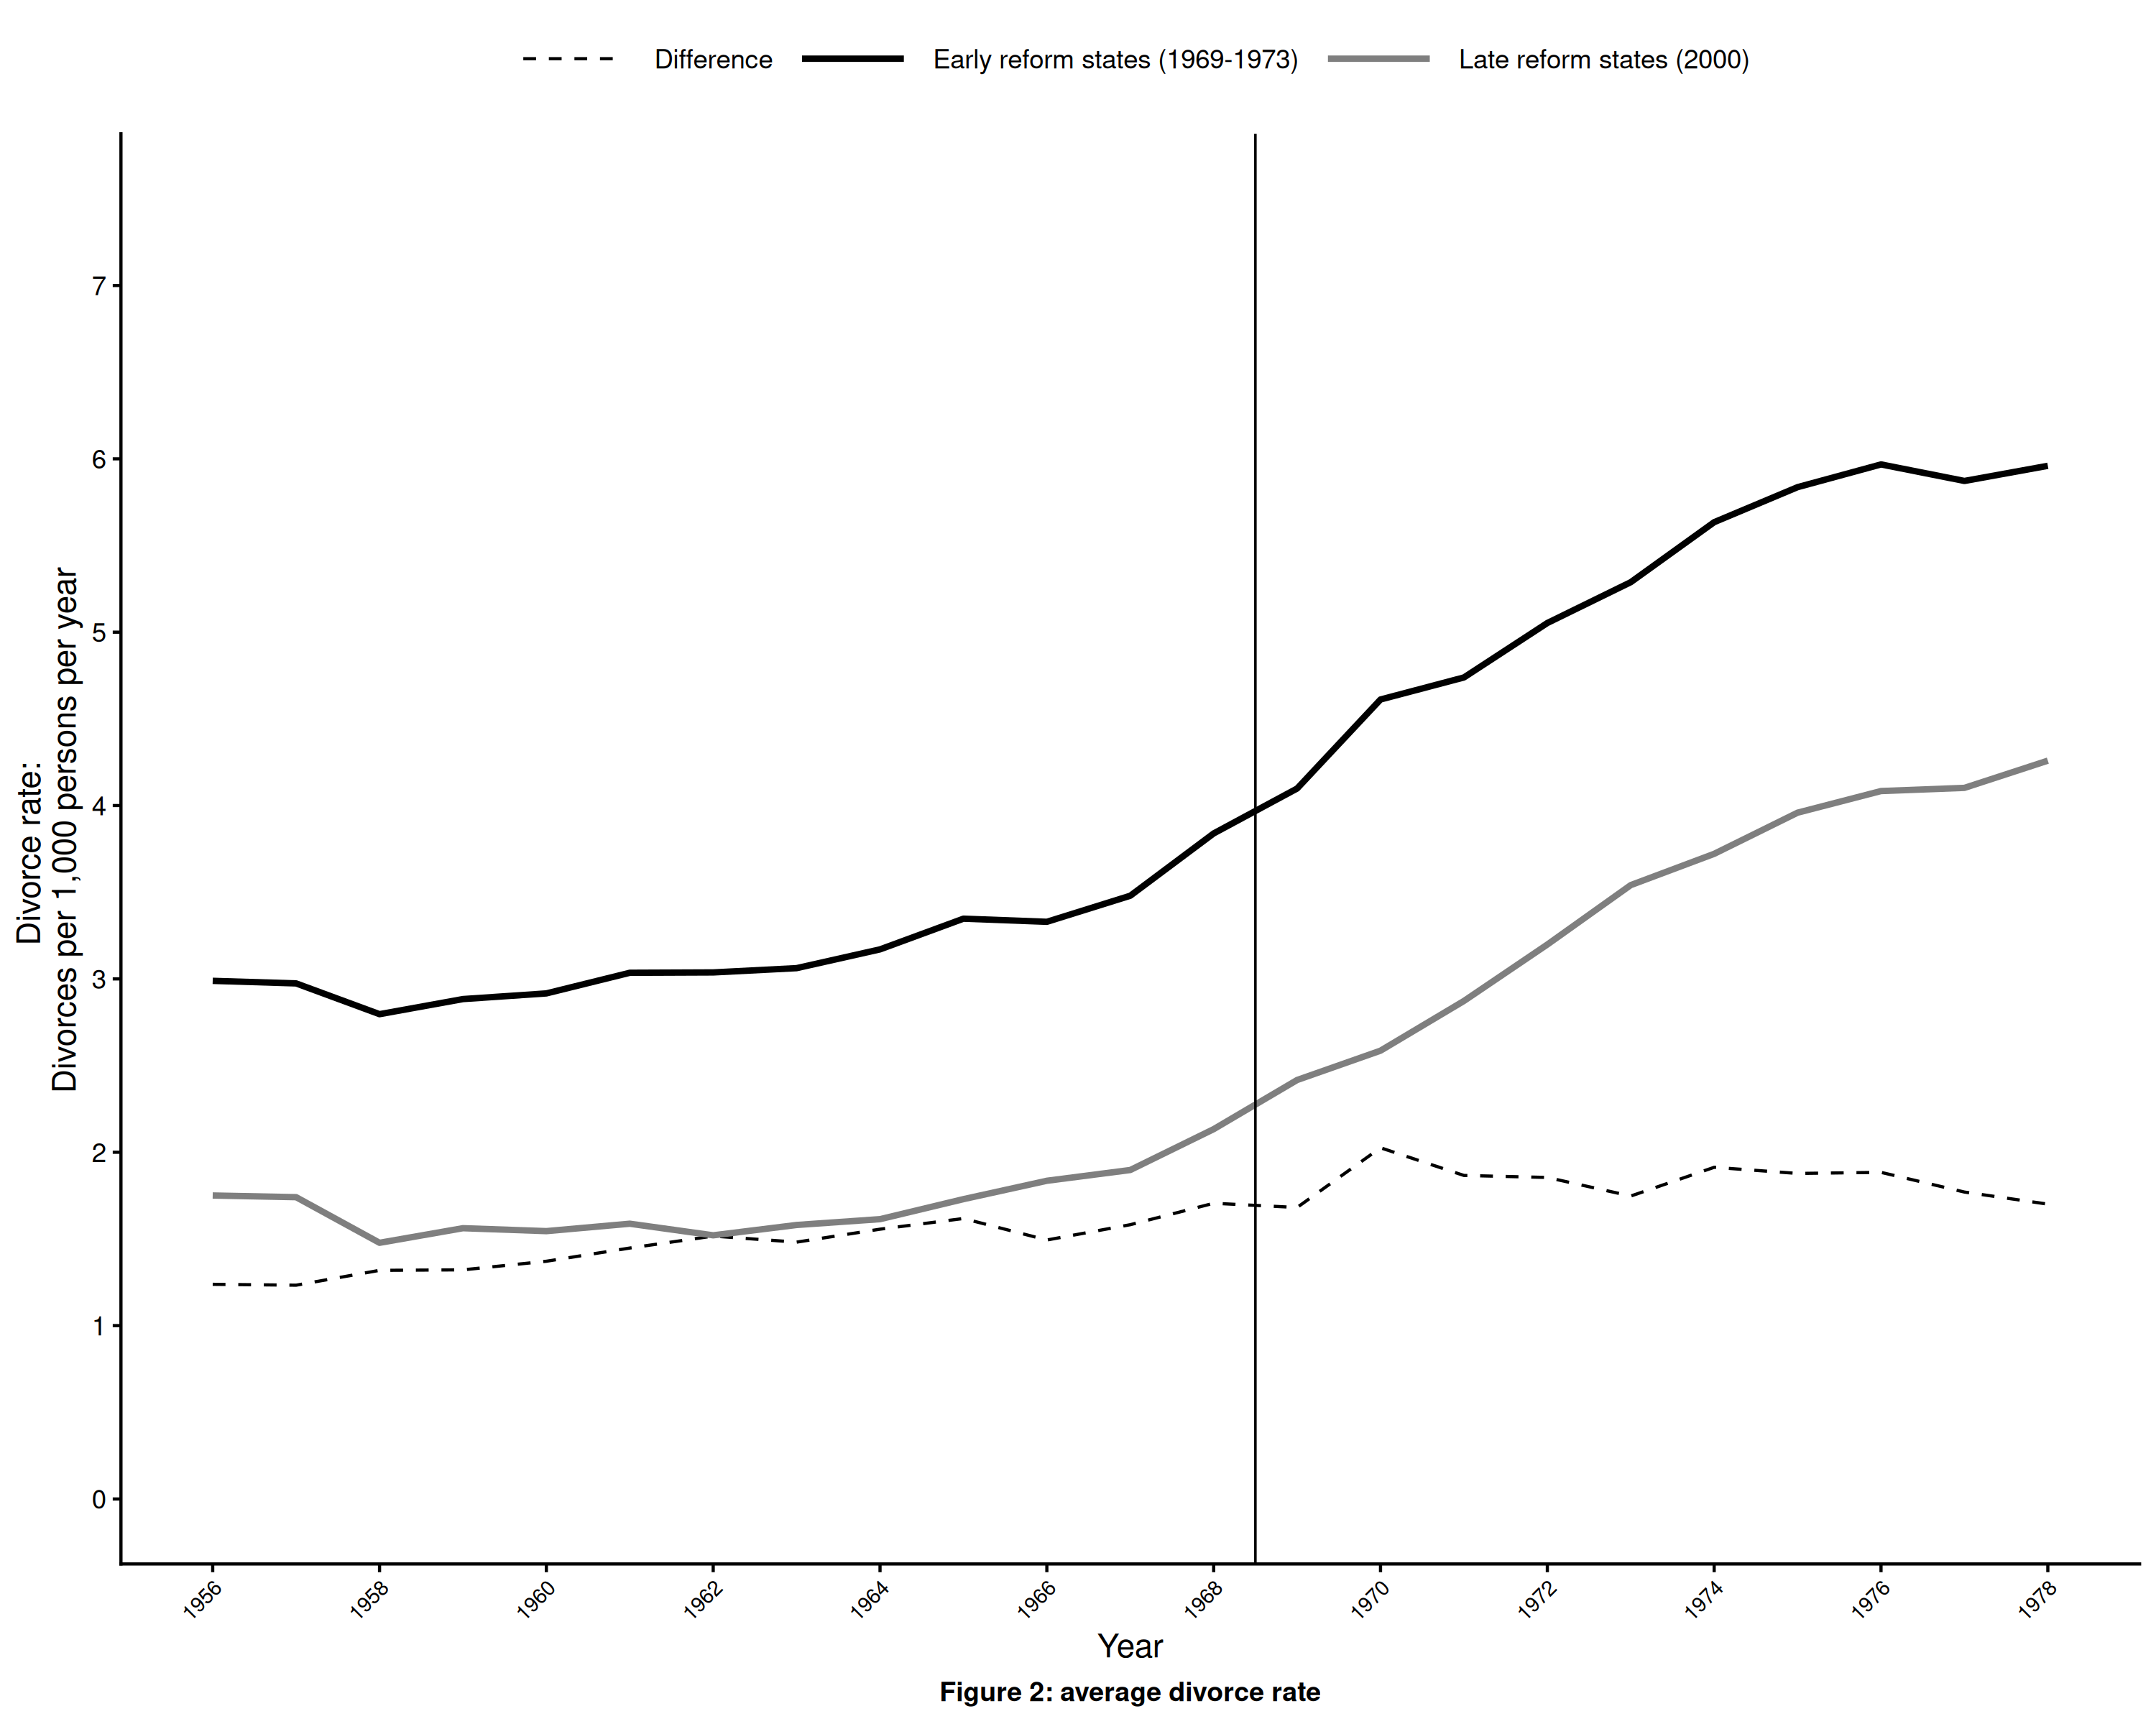
\includegraphics[scale=0.5]{graph2.png}
\end{figure}

\begin{figure}
\centering
\caption{Event study results}
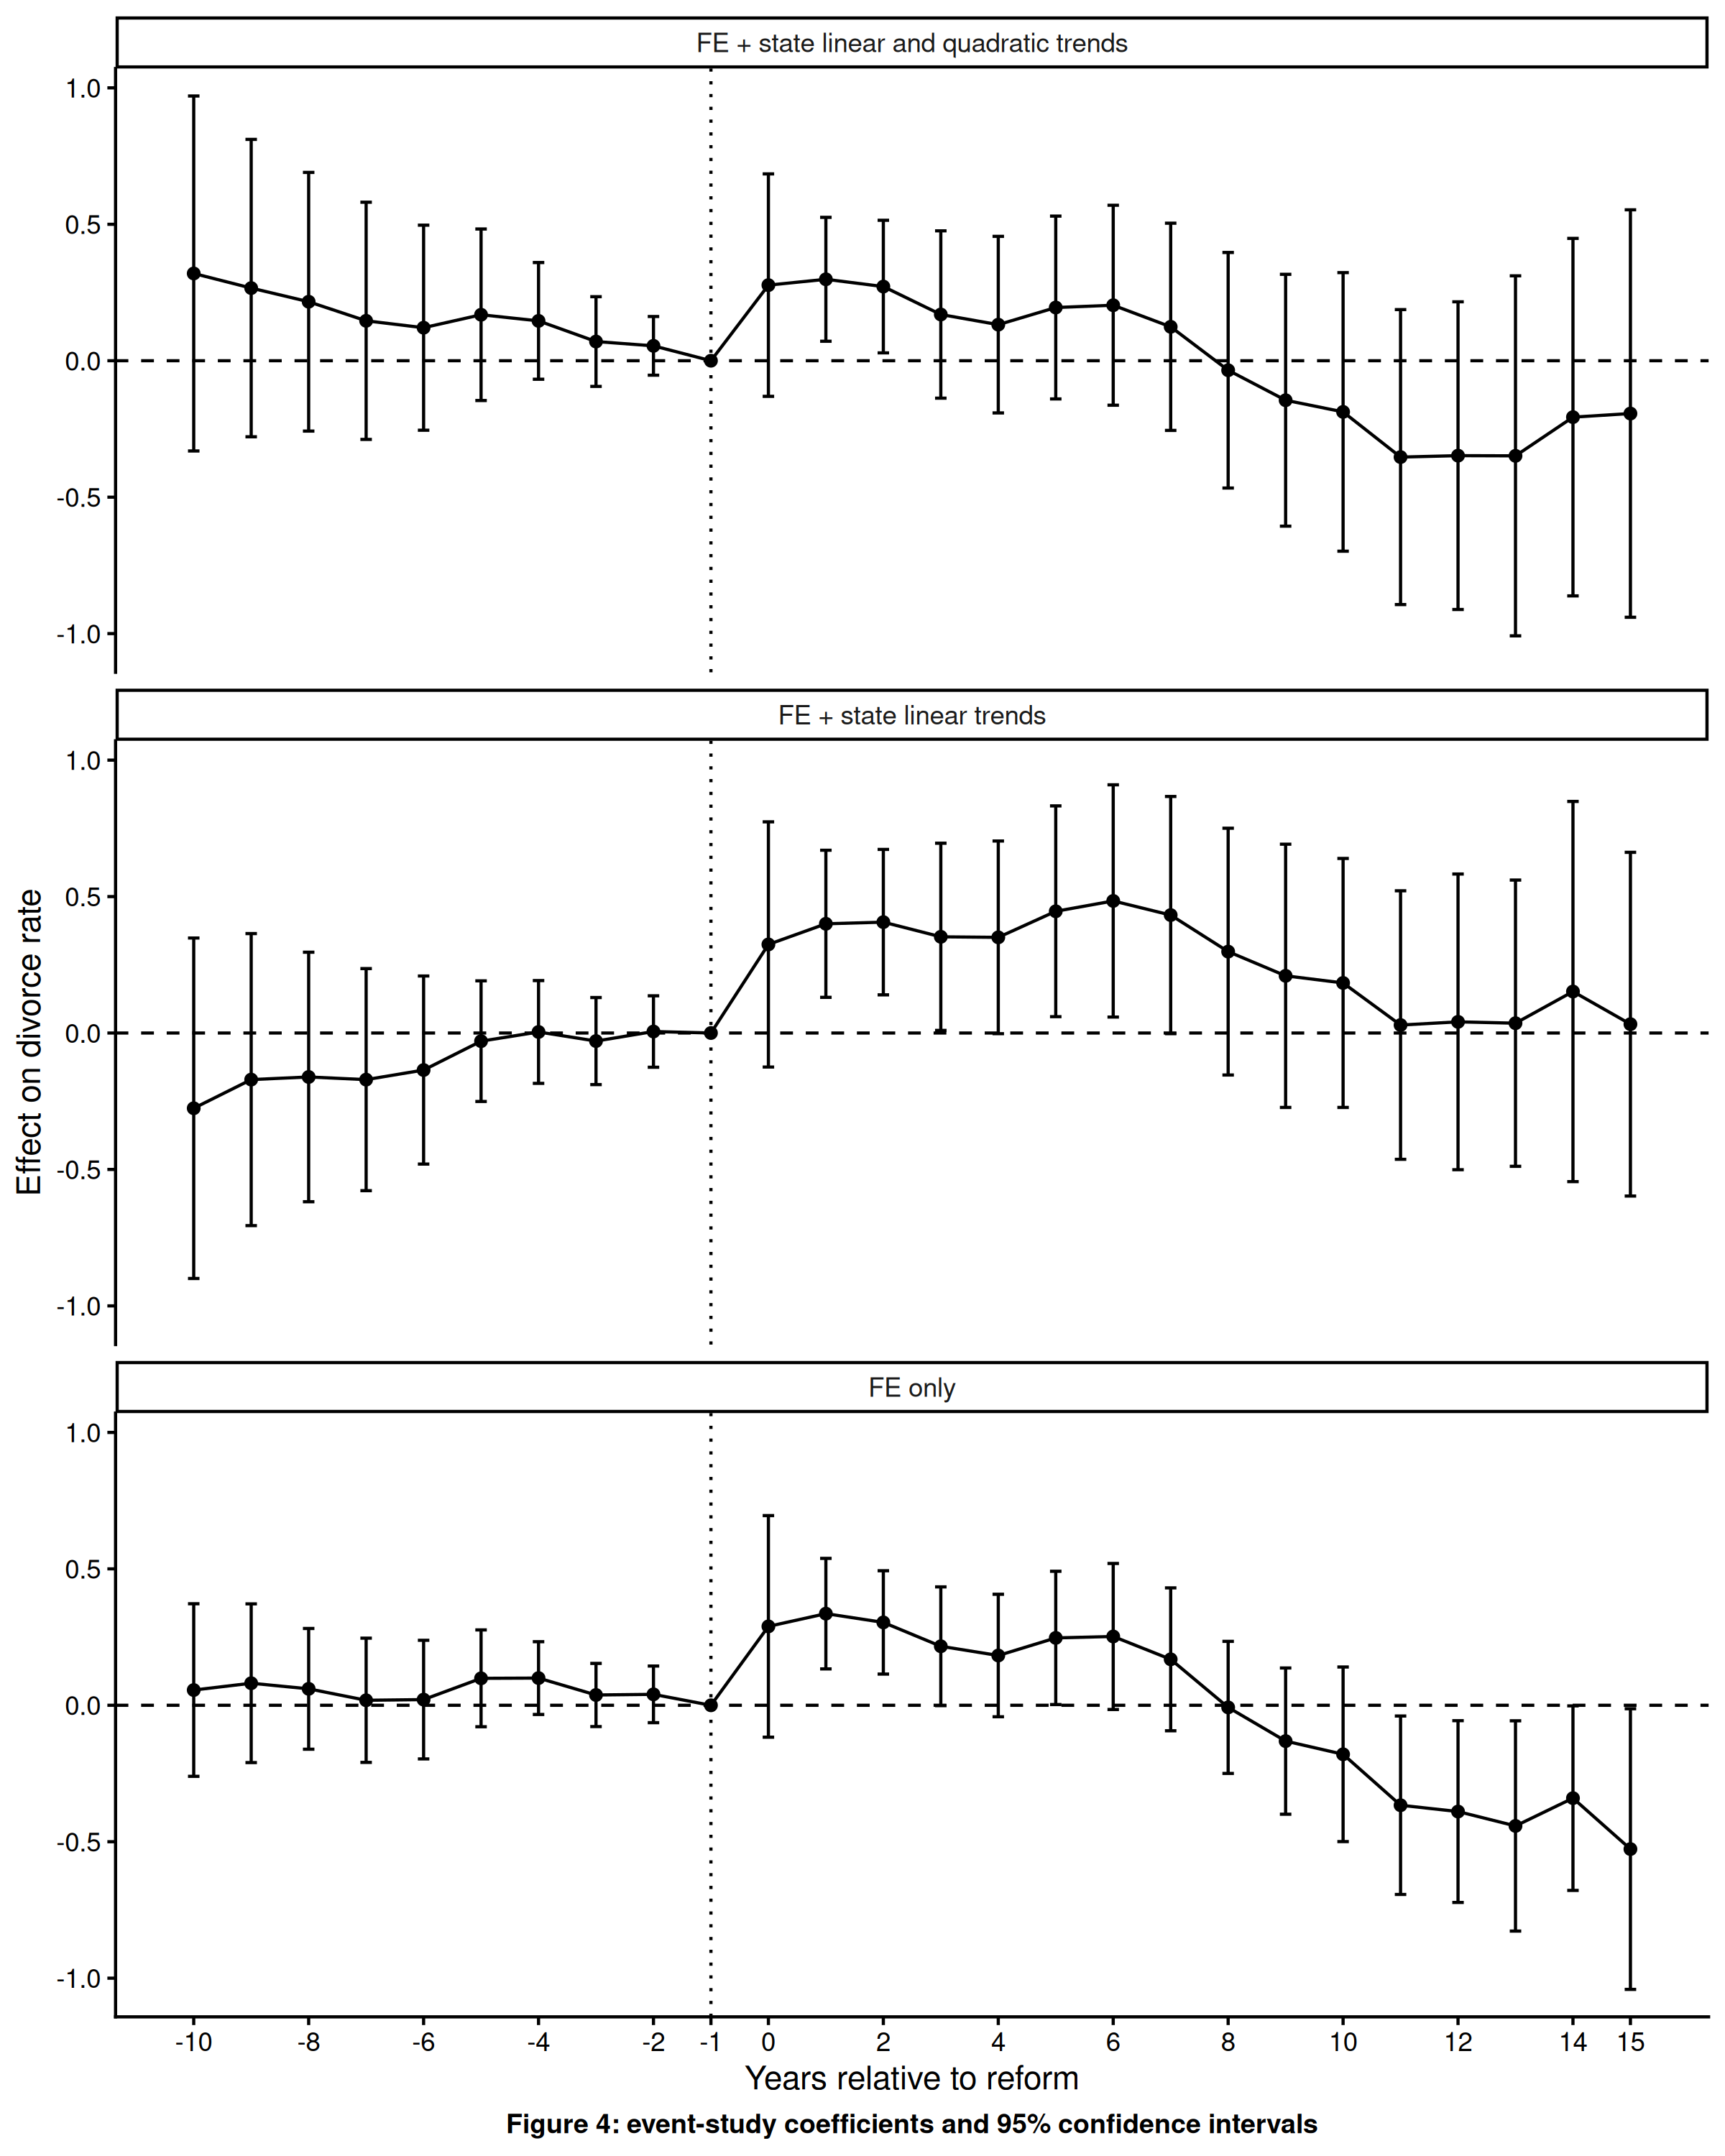
\includegraphics[scale=0.5]{event_study_coefficients.png}
\end{figure}

\begin{figure}
\centering
\caption{Goodman-Bacon decomposition}
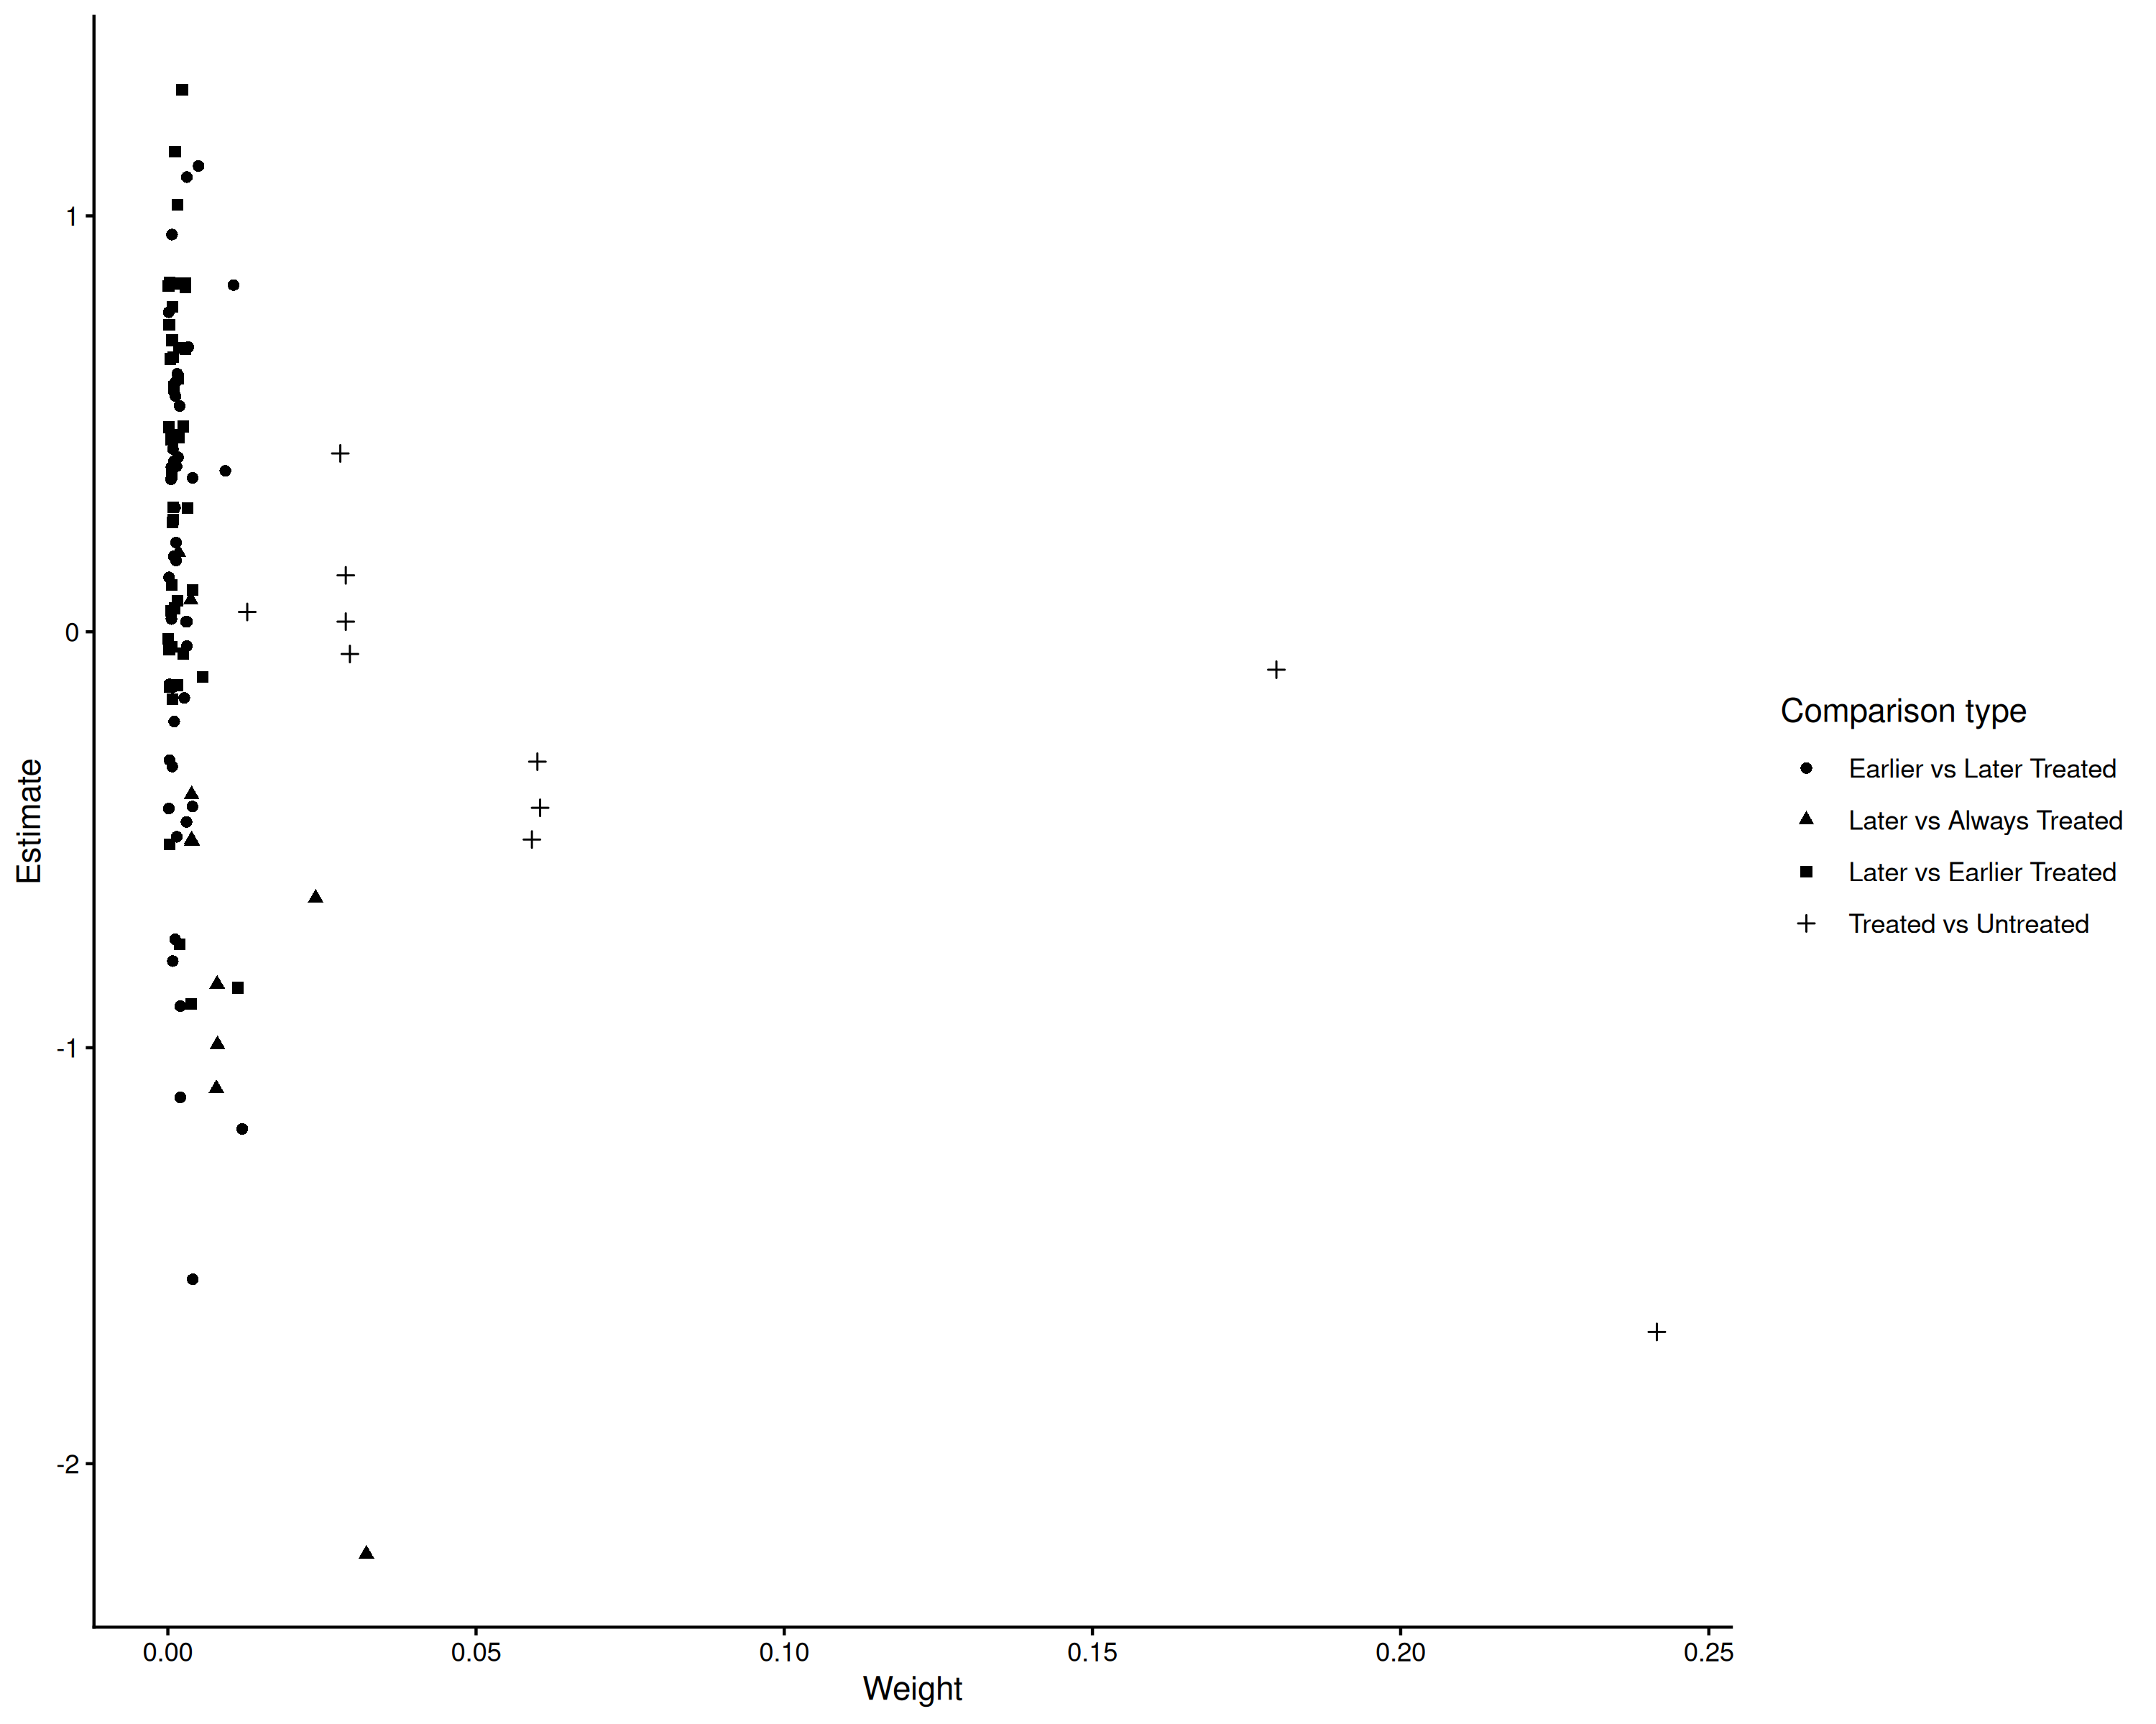
\includegraphics[scale=0.5]{goodmanbacon.png}
\end{figure}

\begin{figure}
\centering
\caption{Sun-Abraham even study results}
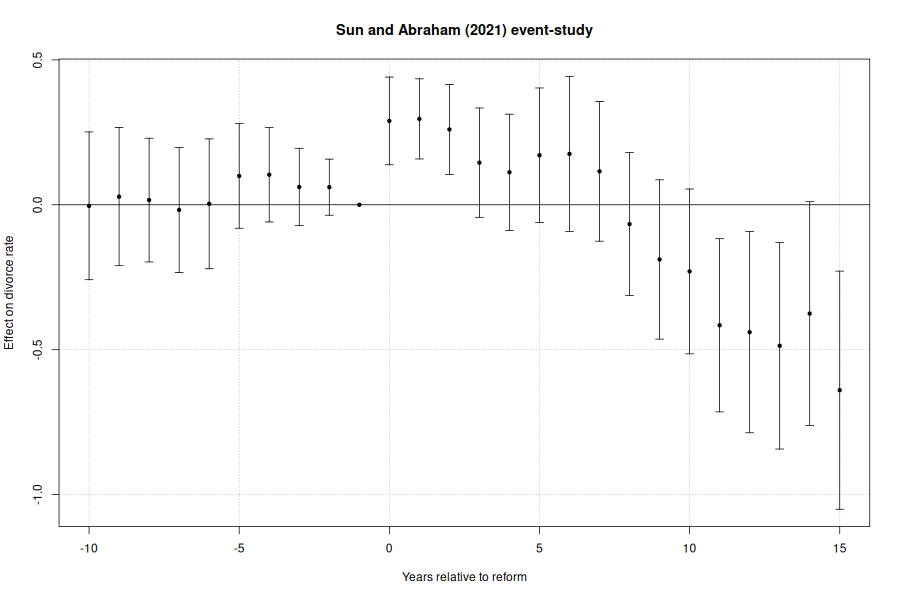
\includegraphics[scale=0.5]{Sun_Abraham_event_study.png}
\end{figure}


% \include{}
% 
% \include{}
% 
% \include{}

\begin{table}[!htbp]\centering
\caption{Causal forest ATE on $\Delta$ divorce rate (1978$-$1968)}
\label{tab:ex2a_ate}
\begin{tabular}{lrrr}
\toprule
Sample & Estimate & Std. Error & t value \\
\midrule
1969-1973 vs 2000 & 0.036 & 0.069 & 0.522 \\
\bottomrule
\end{tabular}
\end{table}


\begin{table}[!htbp]\centering
\caption{Best Linear Projection of CATE on covariates, with AUTOC (Targeting Operator Characteristic area)}
\label{tab:ex2b_blp_toc}
\begin{tabular}{lrrrr}
\toprule
Covariate & Estimate & Std. Error & t value & Pr(>|t|) \\
\midrule
(Intercept) & -1.534 & 0.911 & -1.685 & 0.092 \\
education\_rate\_1968 & 0.004 & 0.006 & 0.725 & 0.469 \\
childcare\_availability\_1968 & 0.031 & 0.251 & 0.124 & 0.902 \\
unemployment\_rate\_1968 & 0.018 & 0.017 & 1.103 & 0.270 \\
median\_income\_1968 & 0.000 & 0.000 & 0.933 & 0.351 \\
urbanization\_1968 & 0.196 & 0.135 & 1.459 & 0.145 \\
marriage\_rate\_1968 & 0.003 & 0.032 & 0.081 & 0.936 \\
religious\_adherence\_1968 & -0.018 & 0.004 & -4.049 & 0.000 \\
alcohol\_consumption\_1968 & 0.005 & 0.020 & 0.231 & 0.817 \\
domestic\_violence\_rate\_1968 & 0.046 & 0.024 & 1.915 & 0.056 \\
women\_labor\_force\_participation\_1968 & 0.018 & 0.007 & 2.683 & 0.007 \\
housing\_cost\_1968 & 0.000 & 0.000 & 0.285 & 0.775 \\
crime\_rate\_1968 & 0.000 & 0.000 & 1.143 & 0.253 \\
social\_services\_spending\_1968 & 0.000 & 0.000 & 0.420 & 0.674 \\
AUTOC (priorities = CATE) & 0.188 & 0.085 & 2.206 & 0.027 \\
\bottomrule
\end{tabular}
\end{table}


\begin{table}[!htbp]\centering
\caption{Effect of disabling honesty: ATE and BLP coefficients}
\label{tab:ex2d_honesty}
\begin{tabular}{lrrrr}
\toprule
Covariate & Honest Est. & Honest SE & No-honesty Est. & No-honesty SE \\
\midrule
ATE & 0.035 & 0.064 & 0.027 & 0.064 \\
(Intercept) & -1.469 & 0.802 & -1.508 & 0.806 \\
education\_rate\_1968 & 0.007 & 0.005 & 0.007 & 0.005 \\
childcare\_availability\_1968 & 0.076 & 0.235 & 0.084 & 0.236 \\
unemployment\_rate\_1968 & 0.019 & 0.014 & 0.019 & 0.014 \\
median\_income\_1968 & -0.000 & 0.000 & -0.000 & 0.000 \\
urbanization\_1968 & 0.191 & 0.131 & 0.170 & 0.132 \\
marriage\_rate\_1968 & 0.008 & 0.027 & 0.009 & 0.028 \\
religious\_adherence\_1968 & -0.016 & 0.004 & -0.015 & 0.004 \\
alcohol\_consumption\_1968 & 0.004 & 0.018 & 0.005 & 0.018 \\
domestic\_violence\_rate\_1968 & 0.036 & 0.020 & 0.034 & 0.020 \\
women\_labor\_force\_participation\_1968 & 0.019 & 0.006 & 0.018 & 0.006 \\
housing\_cost\_1968 & 0.000 & 0.000 & 0.000 & 0.000 \\
crime\_rate\_1968 & 0.000 & 0.000 & 0.000 & 0.000 \\
social\_services\_spending\_1968 & 0.000 & 0.000 & 0.000 & 0.000 \\
\bottomrule
\end{tabular}
\end{table}



\begin{figure}
\centering
\caption{CATEs for the Honest Causal Forest (Exe. 1b)}
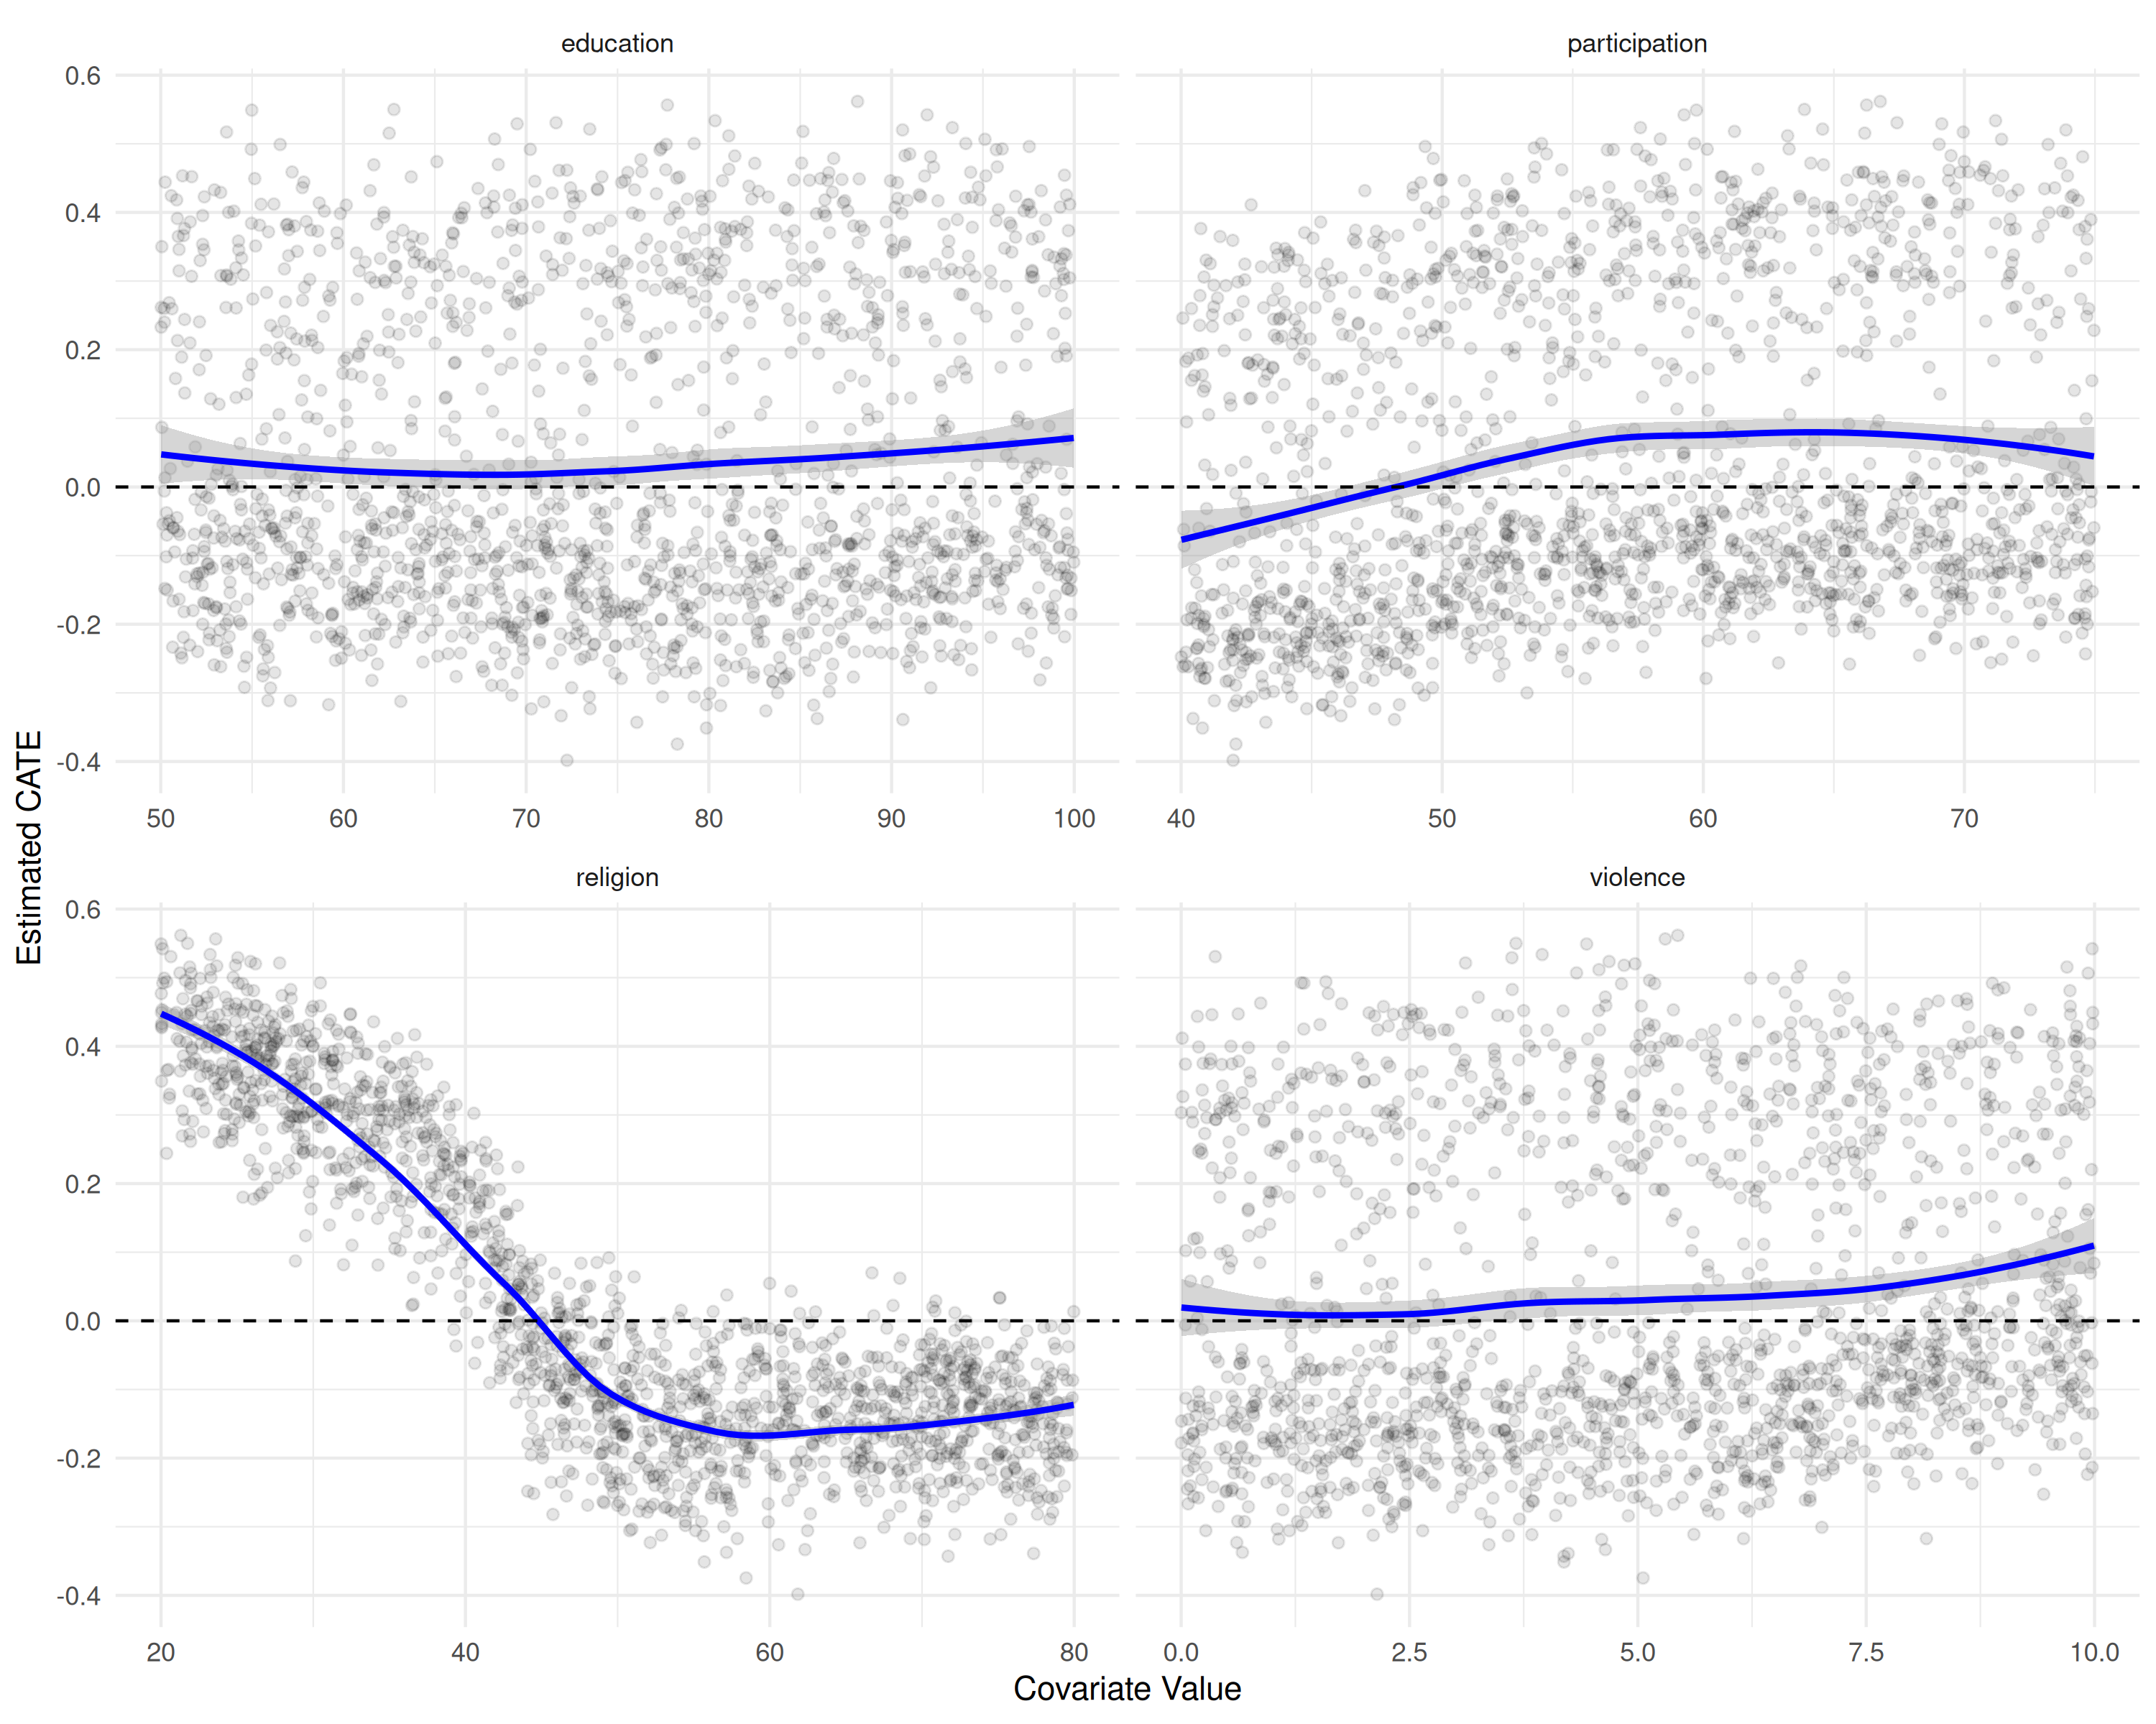
\includegraphics[scale=0.5]{plot_cate.png}
\end{figure}

\begin{figure}
\centering
\caption{CATEs for the Dishonest Causal Forest (Exe. 2d)}
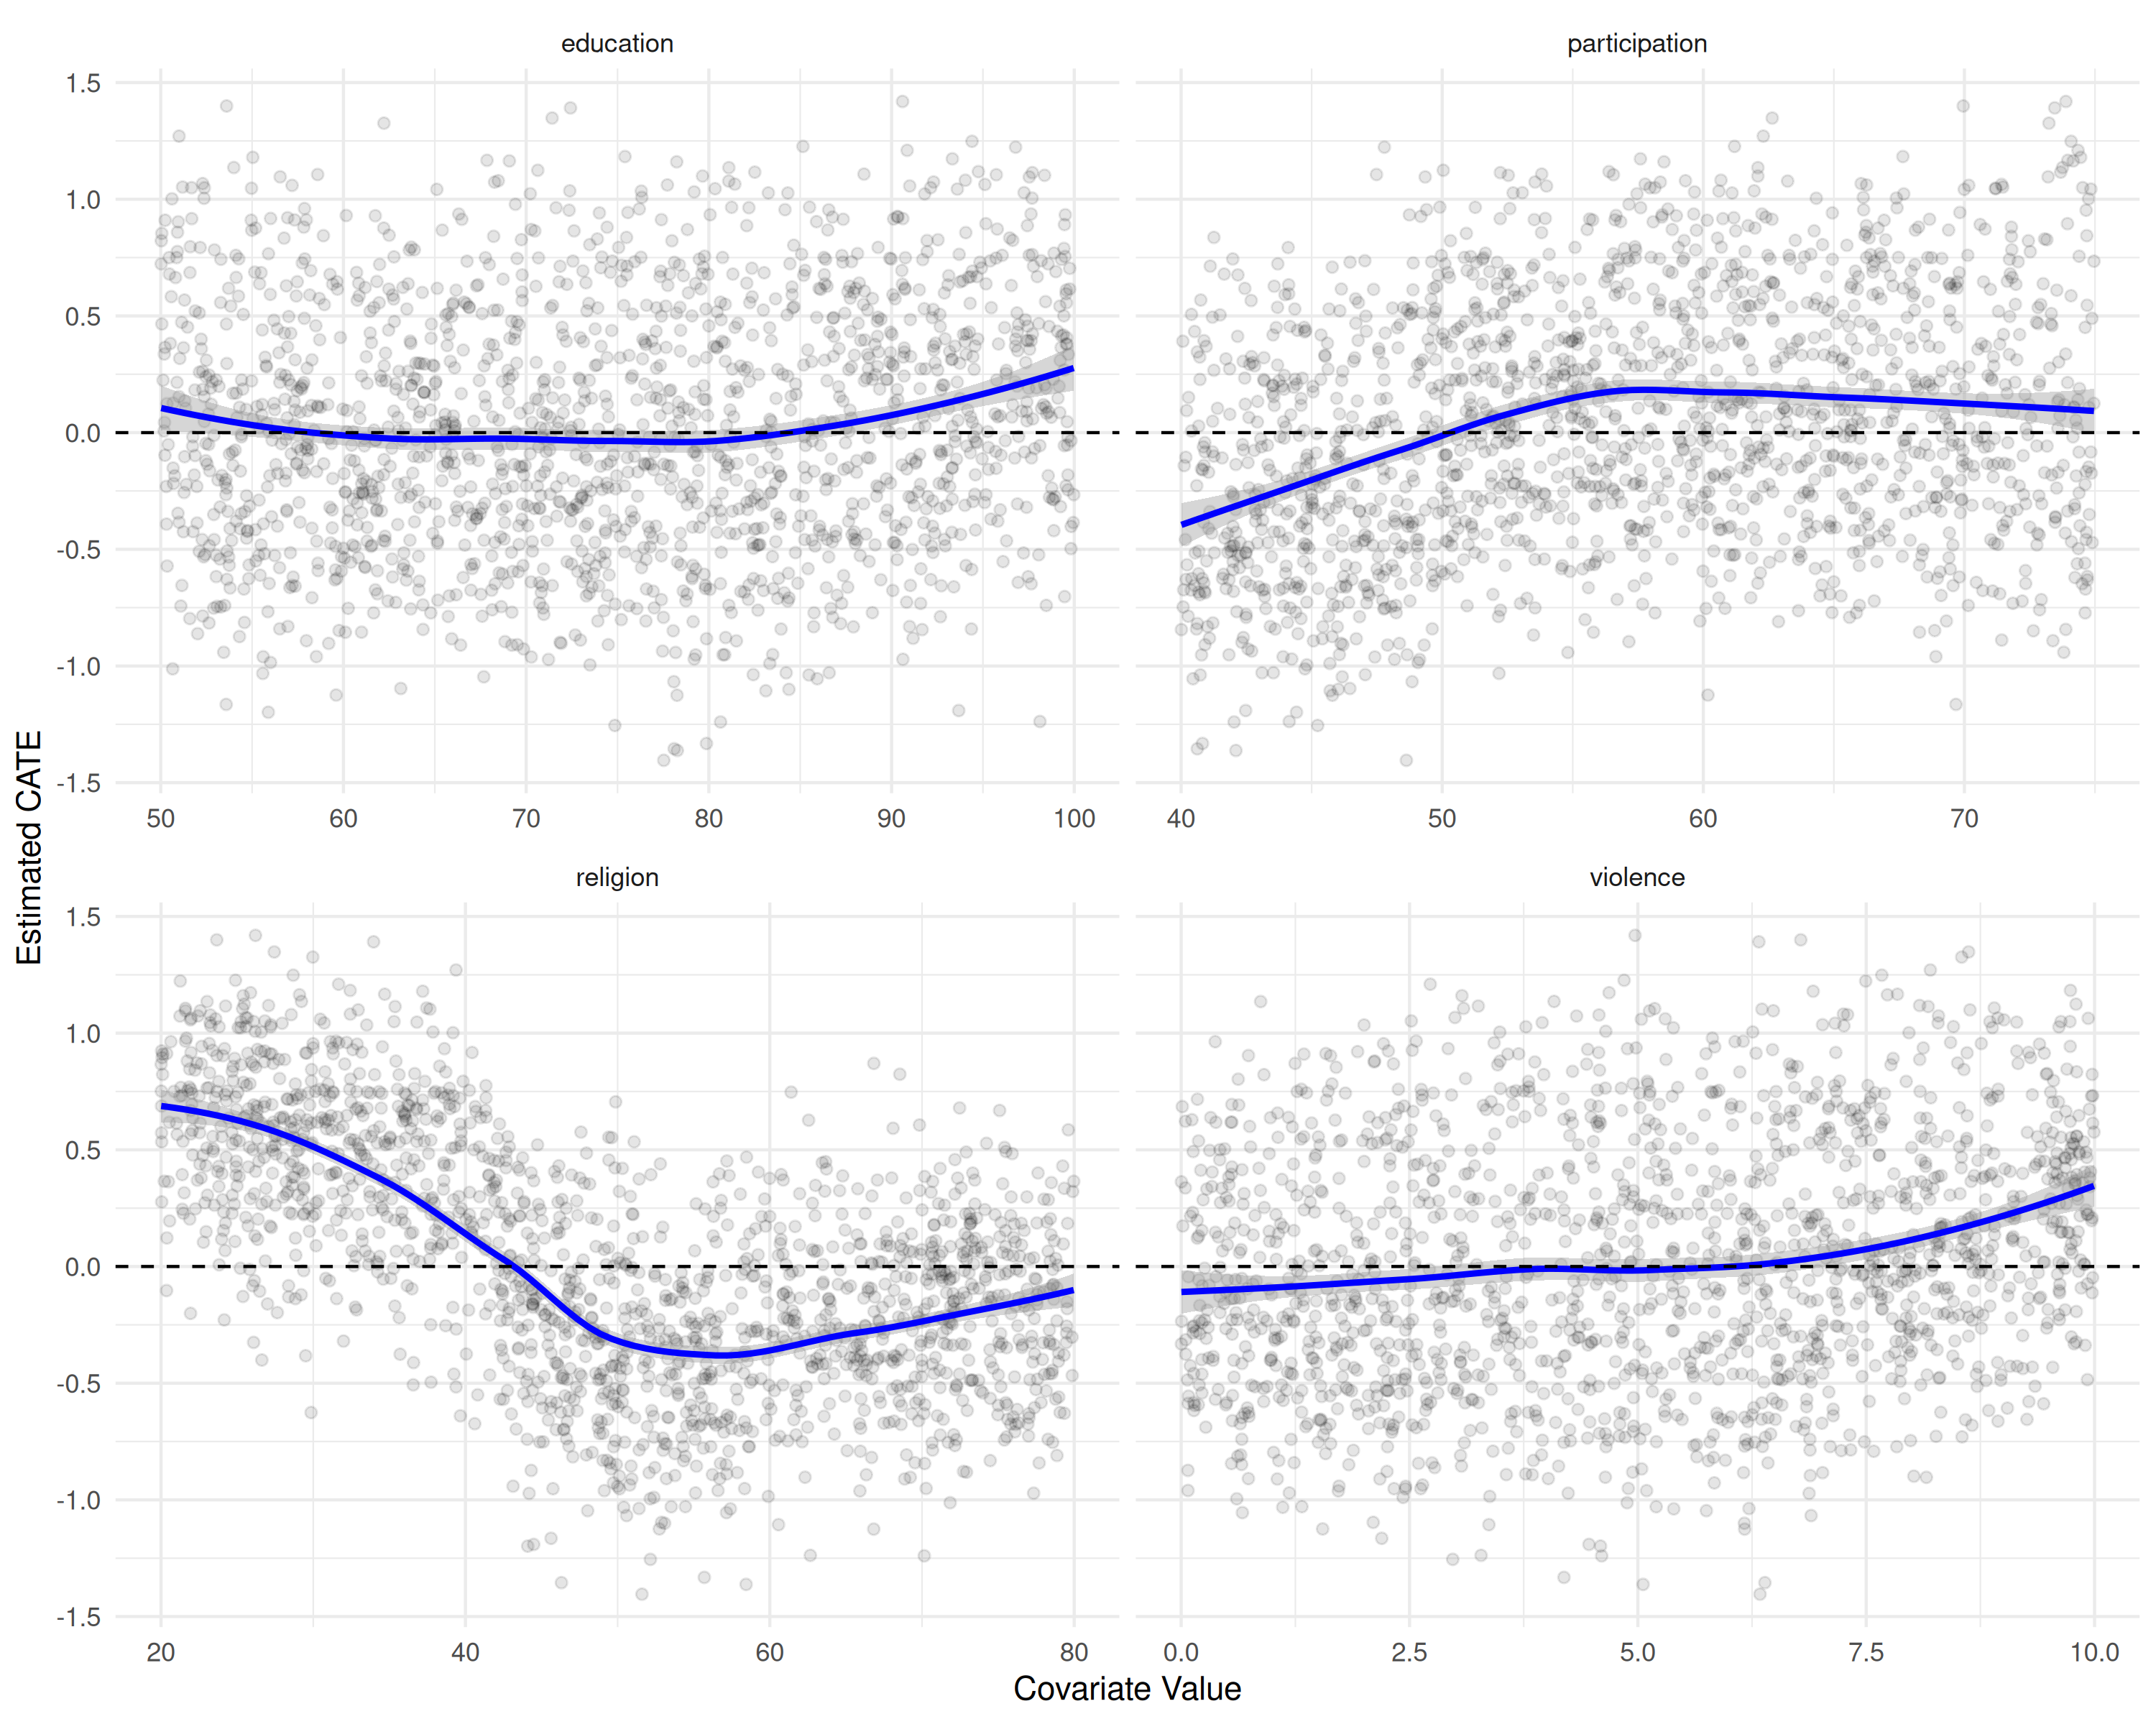
\includegraphics[scale=0.5]{plot_cate_dishonest.png}
\end{figure}


\end{document}
